%%%%%%%%%%%%%%%%%%%%%%%%%%%%%%%%%%%%%%%%%
% NIH Grant Proposal for the Specific Aims and Research Plan Sections
% LaTeX Template
% Version 1.0 (21/10/13)
%
% This template has been downloaded from:
% http://www.LaTeXTemplates.com
%
% Original author:
% Erick Tatro (erickttr@gmail.com) with modifications by:
% Vel (vel@latextemplates.com)
% Michael ma2196@columbia.edu
% with assistance from Jonah G.
% Adapted from:
% J. Hrabe (http://www.magalien.com/public/nih_grants_in_latex.html)
%
% License:
% CC BY-NC-SA 3.0 (http://creativecommons.org/licenses/by-nc-sa/3.0/)
%
%%%%%%%%%%%%%%%%%%%%%%%%%%%%%%%%%%%%%%%%%

%----------------------------------------------------------------------------------------
%	PACKAGES AND OTHER DOCUMENT CONFIGURATIONS
%----------------------------------------------------------------------------------------

\documentclass[11pt,notitlepage]{article}

% A note on fonts: As of 2013, NIH allows Georgia, Arial, Helvetica, and Palatino Linotype. LaTeX doesn't have Georgia or Arial built in; you can try to come up with your own solution if you wish to use those fonts. Here, Palatino & Helvetica are available, leave the font you want to use uncommented while commenting out the other one.

\usepackage{palatino} % Palatino font
%\usepackage{helvet} % Helvetica font
\renewcommand*\familydefault{\sfdefault} % Use the sans serif version of the font
\usepackage[T1]{fontenc}
\linespread{1.05} % A little extra line spread is better for the Palatino font

\usepackage{lipsum} % Used for inserting dummy 'Lorem ipsum' text into the template
\usepackage{amsfonts, amsmath, amsthm, amssymb} % For math fonts, symbols and environments
\usepackage{graphicx} % Required for including images
\usepackage{booktabs} % Top and bottom rules for table
\usepackage{wrapfig} % Allows in-line images
\usepackage[labelfont=bf]{caption} % Make figure numbering in captions bold
\usepackage[top=0.5in,bottom=0.5in,left=0.5in,right=0.5in]{geometry} % Reduce the size of the margin
\pagestyle{empty} % Remove page numbers

\hyphenation{ionto-pho-re-tic iso-tro-pic fortran} % Specifies custom hyphenation points for words or words that shouldn't be hyphenated at all

  
  % to reduce white space between PARAGRAPHS
\setlength{\parskip}{0pt}
\setlength{\parsep}{0pt}

  % additional parameters
%\setlength{\headsep}{0pt}
%\setlength{\topskip}{0pt}
%\setlength{\topmargin}{0pt}
%\setlength{\topsep}{0pt}
%\setlength{\partopsep}{0pt}

  % to reduce white space between SECTIONS
\usepackage[compact]{titlesec}
%\titlespacing{\section}{0pt}{*0}{*0}
%\titlespacing{\subsection}{0pt}{*0}{*0}
%\titlespacing{\subsubsection}{0pt}{*0}{*0}
% \titlespacing{\subparagraph}{0pt}{*0}{*0}
\titlespacing*{\subparagraph} {\parindent}{1ex plus 1ex minus .2ex}{0.5em}


\begin{document}


%----------------------------------------------------------------------------------------
%	SPECIFIC AIMS
%----------------------------------------------------------------------------------------
\part*{Specific Aims}
We propose to improve the prediction and prevention of respiratory failure and death in hospitalized patients by integrating complex Bayesian hierarchical modeling into data acquisition, patient triage and treatment implementation in electronic medical record based (EMR) surveillance.\newline
\textbf{Severe acute respiratory failure (ARF) requiring mechanical ventilation leads to increased mortality,} increased cognitive and functional impairment. EMR surveillance can identify hospitalized patients at risk, days before their deteriorating conditions are typically recognized; earlier initiation of preventive interventions can reduce morbidity, mortality and expenses: My mentor Dr. Gong is leading a randomized multicenter trial to reduce mortality by triggering an individualized prevention checklist for patients identified as at risk. \newline
\textbf{Hierarchical models may perform better than classical models in large data sets} with spatial and temporal organization.
We are particularly interested in fitting complex hierarchical Bayesian models to improve prediction, (1) by allowing model parameters to vary between patients, between medical floors, services or institutions and (2) by modeling variation in compliance and treatment effects during trial implementation. Patients seen by the same team, treated in the same setting or season will show similar clinical trajectories and responses. Especially in the subset with sparse or missing data, precision and accuracy of parameter estimates can be improved by pooling, when they are informed by data from all the other patients. 
\newline \textbf{Heterogeneous provider compliance and missing clinical data may limit implementation} of the prediction algorithm, the therapeutic interventions and the trial itself. I will advance Bayesian data imputation using auxiliary data with Dr. Hall. Seasonal effects and institutional learning may limit prediction accuracy. We will update our model continuously with new patient information, incorporate compliance and effectiveness of the interventions into the model and adjust for seasonal effects in one coherent model.
\newline \textbf{The integration of advanced statistical modeling with EMR surveillance to improve patient outcomes} 
constitutes the unique innovation and power of my proposal. Implementation of Bayesian hierarchical modelling can be computationally challenging for Big Data. My co-mentor Dr. Gelman is leading the NSF-funded development of Stan, statistical software achieving faster convergence and parameter estimation based on novel Markov Chain Monte Carlo computer algorithms. 
\newline \textbf {Under an exceptional and multidisciplinary combination of mentors,} I will integrate complex hierarchical models into an ongoing "real time" EMR based multicenter trial and clinical decision algorithm, advance integrated data imputation and overcome current limitations in Bayesian computational implementation for very large multi-center EMR surveillance. 
\paragraph*{Our overall hypothesis is that complex hierarchical Bayesian modeling and data imputation will reduce morbidity and mortality from respiratory failure in hospitalized patients compared to the classical model.} 

\begin{flushleft}
\textbf{Specific aims:}
\end{flushleft}

\textbf{Aim 1: To improve early prediction of prolonged respiratory failure and death in hospitalized patients.} \newline We will implement a complex hierarchical Bayesian prediction algorithm, comparing it to the classical model. \newline \textbf{SA 1a:} To build a pragmatic EMR based hierarchical Bayesian model implemented in the ultra-fast statistical software Stan to predict a composite outcome [death or prolonged mechanical ventilation > 48 hours] in our Montefiore Medical Center inpatients and compare it with the existing frequentist algorithm. \newline \textbf{SA 1b:} To further develop Bayesian data imputation algorithms of missing clinical data using auxiliary data, to identify the auxiliary measure properties, ceiling and floor effects and to test the imputations against manually verified data and published algorithms.

\textbf{Aims 2: To integrate a complex Bayesian model into patient triage and treatment implementation.} \newline Our prediction algorithm will trigger individualized patient interventions in Dr. Gong's pragmatic multi-center trial. 
\newline \textbf{SA 2a:} To integrate patient triage and advance compliance into Dr. Gong's clinical trial and sustained quality improvement and to focus education efforts on the most effective components of the checklist intervention.
\newline \textbf{SA 2b:} To update our model continuously with new incoming patients, to expand our model to include patients from other regional institutions and to incorporate provider compliance, seasonal effects and institutional learning into the model.

%----------------------------------------------------------------------------------------
%	RESEARCH PLAN
%----------------------------------------------------------------------------------------
\newpage
\part*{Research Plan}

\section*{A. Significance}

\subsection*{Acute respiratory failure is a significant burden of disease for hospitalized patients.}

\subparagraph*{Respiratory failure in hospitalized patients can be predicted and should be prevented}


\subparagraph{Acute respiratory failure is a significant burden of disease.}
Many hospitalized patients develop acute respiratory failure \cite{shinystan}, which is worrisome.

\subsection*{Hierarchical modeling exploits the rich heterogeneity of electronic medical records}

\subparagraph{Electronic medical records are an eminent example of Big Data. }
EMR have more useful data than can be analyzed in a scientifically meaningful way by existing statistical inference tools. This currently limits the scientific hypotheses and clinical inferences, that can be explored and evaluated. Large electronic medical data sets are not just bigger in that there are more instances of the same thing, (this would make data analysis only easier). Rather, there is more breadth to the data: more subgroups, locations, or time granularity than is currently being modeled, more frequent and detailed measurements than can easily be incorporated into standard models, more information on the population units being measured, and more fine-grained information on the predictions desired. EMR are the prime example of a richly structured and correlated web of Big Data.

\subparagraph{Large electronic medical records are nested hierarchically.}
Clinical observations are nested within patients, e.g. repeated glucose measurements will be similar in the same patients. Patients seen by the same provider will have similar outcomes predicted by provider behavior and qualities. Providers are integrated in institutions. Institutions are nested geographically in counties and regions. Health care environments predict patient and provider behavior and outcomes. Patients seen by the same team, treated in the same setting will have similar propensity to respond to interventions. Large electronic medical records require more than just fitting well-known models at larger scales; they requires richer models to exploit fine-grained multilevel structures and to map to predictive questions of interest.

\subparagraph*{Bayesian hierarchical modeling of complex Big Data can be transformative.}
With their inherent flexibility and robustness, Bayesian models may predict better in large data sets with spatial and temporal organization, than classical models \cite{Gelman_red_2009}. Consider our multilevel electronic medical records data set consisting of repeated visits by patients with different ages and medical conditions in different services integrated in different hospitals in different states with different medical plans. Fitting the predictive regression model, we would want the regression coefficients to vary by group (by service, by medical unit, by hospital), to realistically model the complex correlations seen in actual clinical practice: The number of parameters to estimate grows very quickly and so do the potential interactions. Reciprocally, even with very large data sets, the sample size in each subgroup will shrink rapidly; estimates using least squares or maximum likelihood will become noisy and thus often become essentially useless. Regardless, we  will want to estimate various hyper-parameters and hyper-hyper-parameters, to represent how lower level parameters vary across different groupings \cite{Bafumi_Gelman_2007}.

\subparagraph*{"Partial pooling" outperforms the no-pooling and complete-pooling alternatives.}
Hierarchical modeling is more efficient, as can be shown mathematically or via cross-validation \cite{Gelman-Hill_2014}. "No pooling" is one approach to estimate the model for each group separately. Addressing and exploring the complexity and granularity, the richness of the data may lead to far too many sub-classifications, thus too small samples in any given subgroup for useful inferences. "Complete pooling" or structural modeling is another approach, but the implied hard constraints on the coefficients in different groups may lead to bias, in particular for groups with sparse data; we loose information, because we cannot learn from groups where we have more data. In hierarchical modeling, the estimate of each individual parameter is simultaneously informed by data from all the other units; this is what makes "partial pooling" or hierarchical modeling especially effective \cite{Gelman_multilevel_2006}. 

\subparagraph*{Heterogeneous and incomplete clinical data may limit prediction and implementation.}
Variables with strong predictive power in our model may not be recorded in all patients or may be missing for the time window needed for prediction, limiting development of the prediction algorithm, implementation of the therapeutic interventions and the trial itself. To improve prediction for cases with incomplete data, we can impute the missing data. Informative loss by incomplete data may bias risk prediction or may hamper the implementation of the prediction algorithm. Likelihood-based mixed effects models for incomplete data give valid estimates if and only if the data are ignorably missing; that is, the parameters for the missing data process are distinct from those of the main model for the outcome, and the data are missing at random (MAR) \cite{Rubin_1976}. However, this is an unreasonable assumption for our electronic medical records, for example because physicians will request test based on the patients co-morbidity and current clinical conditions. Data will not be missing at random, instead incomplete data will be associated with predictors and outcomes.

\subparagraph*{Auxiliary data can be used to impute incomplete medical records.}
Auxiliary date are additional information available in the form of variables known to be correlated with the missing data of interest. For example, arterial blood gas oxygen saturation may be used to impute peripheral pulse oxymetry or oxygen therapy, if the latter are unavailable for the prediction time window, and vice versa. This approach avoids the perils associated with missing at random (MAR) assumptions, when fitting a non-ignorable missingness model \cite{Wang_20029935}. Adding auxiliary variables not included in the main model for multiple imputation, in other words using additional information that is correlated with the missing outcome is an emerging approach to help correct bias \cite{Meng_1994, Collins_11778676, Rubin_1996}, often relying on Bayesian methods for the multiple imputations approach \cite{Daniels_2008, Schafer_1997}; joint modeling and multiple imputations could both be used also to impute incomplete medical records \cite{Fitzmaurice_2008}. The use of auxiliary data to impute incomplete patient records will improve the prediction model and facilitate smoother implementation of the algorithm into the clinical trial \cite{Hall_25389642}. Moreover, auxiliary data imputation for incomplete electronic medical records is underdeveloped; methodologically, their development is an innovative hallmark of this proposal.

\subparagraph*{Seasonal effects, provider compliance and institutional learning can bias risk prediction.} 
Non-compliance is a major obstacle to the effective delivery of health care and improved outcomes \cite{Duncan_16710766}. The personalized intervention triggered by our EMR-prediction algorithm will only prevent respiratory failure if our physicians and nurses implement them. Improving compliance of health care providers with evidence based interventions continues to be a challenge and is under-researched \cite{Davis_7650822}. Institutional behavior changes in response to trials and quality improvements interventions; patient populations can change over time. Respiratory patients are plagued by seasonal deterioration, which could lead to bias in our model. These seasonal and secular effects will alter the predictors of risk in our model. We will therefore include seasonal effects and continuously update our model with new patient data during the implementation of our trial to account for said changes in the risk profile. The integration of provider compliance, secular and seasonal effects in a EMR triggered pragmatic trial with one coherent model is novel. 

\section*{B. Innovation}
\subparagraph*{Focus on prevention of critical adverse outcomes in hospitalized patients.}
Changes in reimbursement give providers a stake in patient outcomes and led to a keen interest in the prediction and prevention of adverse event in hospitalized patients. It makes sense to focus early intervention on patients at high risk for poor outcomes. This project advances hierarchical Bayesian models to implement this paradigm shift in very large electronic medical records, triggering personalized interventions that drive outcome improvements.

\subparagraph*{Improve imputation of incomplete electronic medical records.}
Incomplete patient data, typical for actual clinical records can hinder the development and execution of our prediction algorithms. We will further Bayesian methods to impute incomplete missing data from additional auxiliary data to overcome this limitation. Beyond improving prediction and patient outcomes in our clinical trial, the Bayesian methods we propose to develop can be employed to impute incomplete electronic medical records in other settings.

\subparagraph*{Integrate critical care with computational statistics.}
To often advances in statistical modeling and clinical science are worlds apart. We want to address a critical problem of scalability in Big Data inference, but are equally motivated by our practical use case, improving our pragmatic clinical trial. The strength of our proposal, therefore, is the integration of disparate disciplines, critical care and computational statistics. 

\subsection*{Summary of the impact}
We tackle a serious health care challenge by integrating advanced hierarchical modeling into a pragmatic clinical trial. Beyond improving morbidity and mortality from respiratory disease in hospitalized patients through improved prediction and prevention, we will develop new methods to impute incomplete electronic medical records from auxillary data and scale Bayesian hierachical models to use in large EMR data. Our proposal is unique and novel in its integration of cutting edge methods from clinical, statistical and computer science to fully realize the promise of Big Data in critical care.

\section*{C. Approach}

\section*{References}

%=======INSTRUCTIONS FOR SIGNIFICANCE==========
\newpage

\section*{A. Significance}

\begin{description} % For subheadings within a section, this template uses the {description} environment, it is not obtrusively large like a \subsection; and facilitates a brief optional subtitle; and it will wrap around figures and tables; it also has a decent amount of whitespace above/below which is less than for a section heading
\item[A.1. Instructions.]{Optional subtitle}
\end{description}

Explain the importance of the problem or critical barrier to progress in the field that the proposed project addresses.

Explain how the proposed project will improve scientific knowledge, technical capability, and/or clinical practice in one or more broad fields.

Describe how the concepts, methods, technologies, treatments, services, or preventative interventions that drive this field will be changed if the proposed aims are achieved.

\begin{description}
\item[A.2. Subheading.]{}
\end{description}

\begin{wraptable}{r}{4.8cm} % Example table with text wrapping around it
\caption{Example Table}
\begin{center}
\begin{tabular}{l l r}
\toprule
\multicolumn{1}{c}{City} & {N\textsuperscript{a}} & {\%Silly}\\
\midrule
San Diego & 289 & 41\%\\
Seattle & 262 & 32\%\\
Galveston & 261 & 15\%\\
St Louis & 269 & 7\%\\
New York & 271 & 4\%\\
Baltimore & 231 & 2\%\\
\emph{Total} & 1,586 & 21\%\\
\hline
\end{tabular}\\
\footnotesize\textsuperscript{a}{All participants clowns.}
\end{center}
\label{default}
\end{wraptable}

\lipsum[8-10]

\begin{wrapfigure}{r}{6.8cm} % Example figure with text wrapping around it
\includegraphics[scale=0.9]{Figures/Fig1.pdf}
\caption{\footnotesize Example wrapped figure. (A) Impressive microscopy image. (B) Impressive data.}
\end{wrapfigure}

\lipsum[5]

\begin{description}
\item[A.3. Another subheading:]{optional subtitle.}
\end{description}

\lipsum[25]

\begin{figure}[b c] % Centered big figure at bottom of the page ([b] argument, could be "t" for top or "h" for here)
\centering
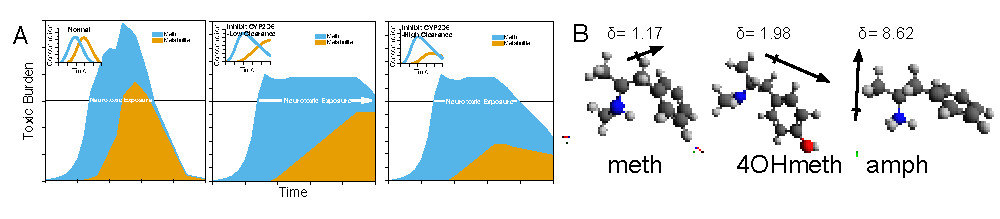
\includegraphics[scale = .80]{Figures/Fig2.pdf}
\caption{\footnotesize Big Figure legend Big Figure legend Big Figure legend Big Figure legend Big Figure legend Big Figure legend Big Figure legend Big Figure legend Big Figure legend.}
\label{fig2}
\end{figure}

\lipsum[31-32]

\begin{description}
\item[A.4. Yet another subheading.]{}
\end{description}

\lipsum[55-56]

%========INSTRUCTIONS FOR INNOVATION================

\section*{B. Innovation}

\begin{description}
\item[B.1. Instructions.]{}
\end{description}

Explain how the application challenges and seeks to shift current research or clinical practice paradigms.

Describe any novel theoretical concepts, approaches or methodologies, instrumentation or interventions to be developed or used, and any advantage over existing methodologies, instrumentation, or interventions.

Explain any refinements, improvements, or new applications of theoretical concepts, approaches or methodologies, instrumentation, or interventions.

%========INSTRUCTIONS FOR APPROACH================

\section*{C. Approach}

\begin{description}
\item[C.1. Instructions.]{}
\end{description}

Describe the overall strategy, methodology, and analyses to be used to accomplish the specific aims of the project. Unless addressed separately in Item 15 (Resource Sharing Plan), include how the data will be collected, analyzed, and interpreted as well as any resource sharing plans as appropriate.

Discuss potential problems, alternative strategies, and benchmarks for success anticipated to achieve the aims.

If the project is in the early stages of development, describe any strategy to establish feasibility, and address the management of any high risk aspects of the proposed work.

Point out any procedures, situations, or materials that may be hazardous to personnel and precautions to be exercised. A full discussion on the use of Select Agents should appear in Item 11, below.

As applicable, also include the following information as part of the Research Strategy, keeping within the three sections listed above: Significance, Innovation, and Approach.

\begin{description}
\item[C.2. Preliminary Studies for New Applications]{}
\end{description}

Preliminary Studies for New Applications: For new applications, include information on Preliminary Studies. Discuss the PD/PI's preliminary studies, data, and or experience pertinent to this application. Except for Exploratory/Developmental Grants (R21/R33), Small Research Grants (R03), and Academic Research Enhancement Award (AREA) Grants (R15), preliminary data can be an essential part of a research grant application and help to establish the likelihood of success of the proposed project. Early Stage Investigators should include preliminary data (however, for R01 applications, reviewers will be instructed to place less emphasis on the preliminary data in application from Early Stage Investigators than on the preliminary data in applications from more established investigators).

%------------------------------------------------

\newpage

\section*{5. Progress Report Publication List (Renewal Applications Only)}

List the titles and complete references to all appropriate publications, manuscripts accepted for publication, patents, and other printed materials that have resulted from the project since it was last reviewed competitively. When citing articles that fall under the Public Access Policy, were authored or co-authored by the applicant and arose from NIH support, provide the NIH Manuscript Submission reference number (e.g., NIHMS97531) or the Pubmed Central (PMC) reference number (e.g., PMCID234567) for each article. If the PMCID is not yet available because the Journal submits articles directly to PMC on behalf of their authors, indicate "PMC Journal -- In Process." A list of these journals is posted at: http://publicaccess.nih.gov/submit\_process\_journals.htm.

Citations that are not covered by the Public Access Policy, but are publicly available in a free, online format may include URLs or PMCID numbers along with the full reference (note that copies of these publications are not accepted as appendix material, see Part I Section 5.5.15 for more information).

%------------------------------------------------

\newpage

\section*{6. Protection of Human Subjects}

Refer to Part II, Supplemental Instructions for Preparing the Human Subjects Section of the Research Plan.

This section is required for applicants answering "yes" to the question "Are human subjects involved?" on the R\&R Other Project Information form. If the answer is "No" to the question but the proposed research involves human specimens and/or data from subjects applicants must provide a justification in this section for the claim that no human subjects are involved.

Do not use the protection of human subjects section to circumvent the page limits of the Research Strategy.

%------------------------------------------------

\newpage

\section*{7. Inclusion of Women and Minorities}

Refer to Part II, Supplemental Instructions for Preparing the Human Subjects Section of the Research Plan. This section is required for applicants answering "yes" to the question "Are human subjects involved?" on the R\&R Other Project Information form and the research does not fall under Exemption 4.

%------------------------------------------------

\newpage

%   \section*{8. Targeted/Planned Enrollment} - form to fill out
\section*{9. Inclusion of Children}

Refer to Supplemental Instructions for Preparing the Human Subjects Section of the Research Plan, Sections 4.4 and 5.7. For applicants answering "Yes" to the question "Are human subjects involved" on the R\&R Other Project Information Form and the research does not fall under Section 4, this section is required.

%------------------------------------------------

\newpage

\section*{10. Vertebrate Animals}

If Vertebrate Animals are involved in the project, address each of the five points below. This section should be a concise, complete description of the animals and proposed procedures. While additional details may be included in the Research Strategy, the responses to the five required points below must be cohesive and include sufficient detail to allow evaluation by peer reviewers and NIH staff. If all or part of the proposed research involving vertebrate animals will take place at alternate sites (such as project/performance or collaborating site(s)), identify those sites and describe the activities at those locations. Although no specific page limitation applies to this section of the application, be succinct. Failure to address the following five points will result in the application being designated as incomplete and will be grounds for the PHS to defer the application from the peer review round. Alternatively, the application’s impact/priority score may be negatively affected.

If the involvement of animals is indefinite, provide an explanation and indicate when it is anticipated that animals will be used. If an award is made, prior to the involvement of animals the grantee must submit to the NIH awarding office detailed information as required in points 1-5 above and verification of IACUC approval. If the grantee does not have an Animal Welfare Assurance then an appropriate Assurance will be required (See Part III, Section 2.2 Vertebrate Animals for more information).
The five points are as follows:

\begin{enumerate}
\item Provide a detailed description of the proposed use of the animals in the work outlined in the Research Strategy section. Identify the species, strains, ages, sex, and numbers of animals to be used in the proposed work.
\item Justify the use of animals, the choice of species, and the numbers to be used. If animals are in short supply, costly, or to be used in large numbers, provide an additional rationale for their selection and numbers.
\item Provide information on the veterinary care of the animals involved.
\item Describe the procedures for ensuring that discomfort, distress, pain, and injury will be limited to that which is unavoidable in the conduct of scientifically sound research. Describe the use of analgesic, anesthetic, and tranquilizing drugs and/or comfortable restraining devices, where appropriate, to minimize discomfort, distress, pain, and injury.
\item Describe any method of euthanasia to be used and the reasons for its selection. State whether this method is consistent with the recommendations of the American Veterinary Medical Association (AVMA) Guidelines on Euthanasia. If not, include a scientific justification for not following the recommendations.
\end{enumerate}

Do not use the vertebrate animal section to circumvent the page limits of the Research Strategy.

%------------------------------------------------

\newpage

\section*{11. Select Agent Research}

Select Agents are hazardous biological agents and toxins that have been identified by DHHS or USDA as having the potential to pose a severe threat to public health and safety, to animal and plant health, or to animal and plant products. CDC maintains a list of these agents. See http://www.cdc.gov/od/sap/docs/salist.pdf.

%------------------------------------------------

\newpage

\section*{12. Multiple PD/PI Leadership Plan}

For applications designating multiple PD/PIs, a leadership plan must be included. A rationale for choosing a multiple PD/PI approach should be described. The governance and organizational structure of the leadership team and the research project should be described, including communication plans, process for making decisions on scientific direction, and procedures for resolving conflicts. The roles and administrative, technical, and scientific responsibilities for the project or program should be delineated for the PD/PIs and other collaborators.

If budget allocation is planned, the distribution of resources to specific components of the project or the individual PD/PIs should be delineated in the Leadership Plan. In the event of an award, the requested allocations may be reflected in a footnote on the Notice of Grant Award.

%------------------------------------------------

\newpage

\section*{13. Consortium/Contractual Arrangements}

Explain the programmatic, fiscal, and administrative arrangements to be made between the applicant organization and the consortium organization(s). If consortium/contractual activities represent a significant portion of the overall project, explain why the applicant organization, rather than the ultimate performer of the activities, should be the grantee. The signature of the Authorized Organization Representative on the SF424 (R\&R) cover component (Item 17) signifies that the applicant and all proposed consortium participants understand and agree to the following statement:

\emph{The appropriate programmatic and administrative personnel of each organization involved in this grant application are aware of the agency's consortium agreement policy and are prepared to establish the necessary inter-organizational agreement(s) consistent with that policy.}

%------------------------------------------------

\newpage

%   \section*{14. Letters of Support} - letters to attach
\section*{15. Resource Sharing}

NIH considers the sharing of unique research resources developed through NIH-sponsored research an important means to enhance the value and further the advancement of the research. When resources have been developed with NIH funds and the associated research findings published or provided to NIH, it is important that they be made readily available for research purposes to qualified individuals within the scientific community. See Part III, 1.5 Sharing Research Resources.

\begin{enumerate}
\item{Data Sharing Plan:} Investigators seeking \$500,000 or more in direct costs (exclusive of consortium F\&A) in any year are expected to include a brief 1-paragraph description of how final research data will be shared, or explain why data-sharing is not possible. Specific Funding Opportunity Announcements may require that all applications include this information regardless of the dollar level. Applicants are encouraged to read the specific opportunity carefully and discuss their data-sharing plan with their program contact at the time they negotiate an agreement with the Institute/Center (IC) staff to accept assignment of their application. See Data-Sharing Policy or http://grants.nih.gov/grants/guide/notice- files/NOT-OD-03-032.html.
\item{Sharing Model Organisms:} Regardless of the amount requested, all applications where the development of model organisms is anticipated are expected to include a description of a specific plan for sharing and distributing unique model organisms or state why such sharing is restricted or not possible. See Sharing Model Organisms Policy, and NIH Guide NOT-OD-04-042.
\item{Genome Wide Association Studies (GWAS):} Applicants seeking funding for a genome-wide association study are expected to provide a plan for submission of GWAS data to the NIH-designated GWAS data repository, or an appropriate explanation why submission to the repository is not possible. GWAS is defined as any study of genetic variation across the entire genome that is designed to identify genetic associations with observable traits (such as blood pressure or weight) or the presence or absence of a disease or condition. For further information see Policy for Sharing of Data Obtained in NIH Supported or Conducted Genome-Wide Association Studies, NIH Guide NOT-OD-07-088, and http://grants.nih.gov/grants/gwas/.
\end{enumerate}


%----------------------------------------------------------------------------------------
%	BIBLIOGRAPHY
%----------------------------------------------------------------------------------------

\newpage

\bibliography{K01_bibliography_7Feb15} % Use the NIHbibliography.bib file for the reference list; the file name cannot contain spaces
\bibliographystyle{nihunsrt} % Use the custom nihunsrt bibliography style included with the template

%----------------------------------------------------------------------------------------

\end{document} 
